\chapter{\leavevmode \newline Conclusion and Future Work}
\label{chap:Discussion}

\section{Conclusion}

This thesis presented a novel navigation framework for proprioceptive terrain-aware exploration in granular environments, where conventional visual sensing is unreliable or unavailable. The system was designed to address the core challenges of uncertainty, deformability, and incomplete knowledge that arise in planetary terrain scenarios. By integrating Gaussian Process-based terrain modeling, confidence-guided safe set expansion, and diffeomorphic reactive control, \algoname\ enables legged robots to safely and adaptively explore unknown environments using only local physical interaction.

Through simulation-based validation, \algoname\ demonstrated three key capabilities: safely navigating around high-risk terrain, efficiently reusing previously learned safe paths, and rapidly expanding known terrain through exploratory behavior. Unlike prior approaches that rely on global visual maps or precomputed paths, \algoname\ achieves safety-aware navigation using real-time proprioceptive measurements and confidence-aware planning, filling a critical gap in current planetary robotics literature.

This work contributes a unified framework for autonomous, local-information-driven exploration under risk constraints, opening new possibilities for robotic operation in visually degraded and mechanically unstable environments.

\section{Future Work}

While the proposed method successfully addresses many core challenges, several directions remain open for further enhancement and investigation.

\subsection{Adapting the Kernel Model for Terrain-Specific Exploration}

One limitation of the current system lies in the use of a radial basis function (RBF) kernel with a fixed length scale. Although this kernel captures smooth terrain correlations effectively, it assumes spatial homogeneity across the entire domain. In practice, terrain conditions often vary dramatically—some areas may require finer resolution due to localized instability, while others may permit broader generalization.

To address this, future work could explore the use of attentive or adaptive kernels \cite{chen2022akattentivekernelinformation} that dynamically adjust the kernel length scale based on local terrain variation or uncertainty. This would allow \algoname\ to quickly sweep through regions of low complexity while cautiously probing areas with steep gradients or sparse data. Such local adaptivity may reduce sampling requirements and improve both efficiency and safety in real-world deployments.

\subsection{Bayesian Planning to Avoid Frontier Oscillation}

Another improvement involves extending the planning strategy beyond the current greedy sampling approach. At present, \algoname\ selects the next expander point based on the highest local uncertainty, which can lead to inefficient "zig-zagging" behavior when traversing across a discrete frontier of uncertain terrain. This behavior, illustrated in \autoref{fig:zig-zag}, arises because uncertainty is reduced only in the immediate vicinity of each expander, causing its neighbors momentarily become the new most uncertain.

\begin{figure}[h]
    \centering
    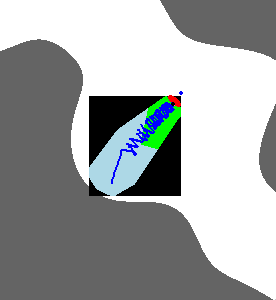
\includegraphics[width=0.5\linewidth]{figures/zigzag.png}
    \caption{"Zig-Zag" behavior of the robot when searching in a straight line.}
    \label{fig:zig-zag}
\end{figure}

To overcome this limitation, future versions of \algoname\ could incorporate probabilistic or belief-space planning frameworks, such as partially observable Markov decision processes (POMDPs). These models consider both the robot’s current knowledge and its uncertainty over future terrain, allowing actions to be chosen based on expected long-term information gain or goal reachability. Rather than selecting the immediate best expander point, the robot could simulate sequences of actions that maximize the likelihood of expanding the frontier coherently or reaching a distant goal safely.

Such methods would reduce redundant sampling and promote smoother, more globally directed navigation. Ultimately, this integration could yield an exploration strategy that balances near-term caution with long-term progress, improving performance in both open and constrained terrains.

\subsection{Integration with Exteroceptive Sensing to Include Planning for Physical Obstacles}

While \algoname\ excels at evaluating terrain risk through proprioceptive interaction, it currently assumes that all safe areas are also free of physical obstructions. In practical planetary scenarios, however, safe terrain may still contain non-traversable obstacles such as rocks, outcrops, or structural debris. These features are often static, geometrically well-defined, and perceptible through standard sensing modalities such as stereo vision, LiDAR, or depth cameras—even in partially degraded visual conditions.

Future work could enhance the current framework by integrating conventional exteroceptive sensors to build geometric representations of physical obstacles within the safe set. By fusing proprioceptive terrain safety maps with geometric occupancy grids or semantic segmentation outputs, the robot could distinguish between terrain that is merely risky (e.g., soft or unstable) and terrain that is physically blocked. This would allow for more nuanced path planning decisions—for instance, avoiding areas that are both risky and cluttered, while still exploring marginally risky but obstacle-free terrain.

Furthermore, this integration would enable multi-layered constraint handling within the local control policy. The diffeomorphic mapping currently used to avoid terrain-based obstacles can be used to encode hard geometric constraints derived from point cloud clustering or shape modeling. 

Incorporating geometric obstacle information  opens the door to hybrid planning techniques, where a higher-level geometric planner filters feasible corridors while \algoname\ locally selects among those corridors based on proprioceptive risk. This two-tiered approach could significantly improve global efficiency, especially in cluttered environments where terrain risk alone does not fully constrain the robot’s motion.

Together, these enhancements would elevate \algoname\ from a proprioceptive-only planner to a more complete terrain-aware motion planning framework, capable of leveraging multiple sensing modalities to ensure both geometric and mechanical safety.